\section{Paketdetails}
\begin{figure}[H]
\centering
\includegraphics[height=0.75\linewidth, angle=90]{img/7-paketdetails}
\caption{Klassendiagramm zur detaillierten Beschreibung der strukturellen Gliederung}
\label{Paketdetails}
\end{figure}
%\pagebreak

%7.1 Paket Robot
\subsection{Paket \textit{RobotUnit}}
	Im Folgenden beschreiben wir die elementaren Klassen des Pakets \textit{RobotSoftware} 
	und ihre zugehörigen wichtigsten Methoden, sowie ihre Interaktion untereinander. 


	%7.1.1 RobotController
	\subsubsection{Beschreibung der Klasse \textit{RobotController}}
%		\begin{figure}[H]
%		\centering
%		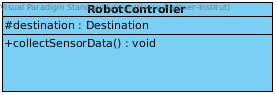
\includegraphics[width=0.6\textwidth]{../images/Iteration0_Entwurf_7-1-1_Klasse_RobotController}
%		\caption{\textcolor{blue}{Durch eigene Diagramme ersetzen}}
%		\label{BeschreibungKlasse1}
%		\end{figure}
		
		%#destination : Destination
		Die Klasse \textit{RobotController} ist die Hauptklasse der \textit{RobotSoftware}, 
		da sie den aktuellen Zustand der \textit{RobotUnit} kapselt.
		Sie verwaltet alle internen Vorgänge der \emph{RobotUnit} und speichert den gerade verfolgten \textit{Task}. Dabei gibt es drei mögliche Zustände: 1. Die \emph{RobotUnit} verfolgt eine vom \emph{Server} auferlegte \emph{Task}. 2. Die \emph{RobotUnit} hat sich selbstständig den \emph{Task} gegeben, einen \emph{Charger} aufzusuchen. 3. Es gibt derzeit keinen \emph{Task}.

			%7.1.1.1 #collectSensorData():void
			\paragraph{Beschreibung der Methode \texttt{readSensors}}
			Der Server kann eine \textit{RobotUnit} dazu auffordern, ihm seine Sensordaten zu schicken. 
			Die \textit{RobotUnit} fragt dann seine Hardwareschnittstelle mittels der Methode \texttt{readSensors} 
			nach seiner Position und seinem Akkustand an und gibt diese Informationen zurück an den \textit{Server}. 
			Dazu wird natürlich zunächst eine \textit{Message} verfasst, welche dann über den \textit{IWlanAdapter} verschickt wird.
			
			\paragraph{Beschreibung der Methode \texttt{setTask}}
			Diese Methode wird aufgerufen, wenn die \textit{RobotUnit} einen neuen Task erhält. Wenn der \textit{Robot} davor keinen \textit{Task} hatte, wird dieser einfach ausgeführt. Wenn der übergebene \textit{Task} \texttt{null} ist, nimmt die \textit{RobotUnit} fahrt zur Ladestation auf. Wenn die \textit{RobotUnit} gerade einen \textit{TaxiCustomer} an Bord hat und in dieser Methode einen Krankenhaustransport als \textit{Task} erhält, wird der \textit{TaxiCustomer} abgeladen, und der Krankenhaustransport wird ausgeführt.
			
			\paragraph{Beschreibung der Methode \texttt{calculateObstaclePosition}}
			Sobald die geringste Distanz eines der IR-Sensoren eines Roboters die Minimaldistanz \texttt{MIN\_IR\_DISTANCE} unterschreitet, soll mittels \texttt{driveAroundObstacle} das erkannte \emph{Obstacle} umfahren werden. Um für die \texttt{driveAroundObstacle}-Methode eine Position angeben zu können, muss jedoch zunächst die Position des \emph{Obstacles} errechnet werden.
			
			Dazu wird in der Methode \texttt{calculateObstaclePosition} mittels folgender mathematischer Berechnungen die Position des \emph{Obstacles} errchnet:
			
			\begin{align*}
				x &= \texttt{currentPosition.x} + cos(\texttt{positionDegree()}) \cdot \texttt{distance()} \\
				y &= \texttt{currentPosition.y} + sin(\texttt{positionDegree()}) \cdot \texttt{distance()}
			\end{align*}
			
			Wurde die Position des \emph{Obstacles} berechnet, wird sie von der Methode \texttt{calculateObstaclePosition} zurückgegeben.
			
	\subsubsection{Beschreibung der Klasse \textit{VirtualServer}}
	Die Klasse \textit{VirtualServer} ist die Klasse, welche die Remote-Procedure-Calls von der Seite der \textit{RobotUnit} implementiert. \textit{VirtualServer} implementiert unsere in Kapitel 3. definierten Interfaces \textit{IRepair} und \textit{IArrivalNotification}. Alle Methoden in dieser Klasse verfassen natürlich eine \textit{Message} und nutzen dann die \textit{IWlanAdapter}-Schnittstelle, um diese an den \textit{Server} zu schicken.
	
			\paragraph{Beschreibung der Methode \texttt{informAboutArrival}}
			Diese Methode wird immer dann aufgerufen, wenn die \textit{RobotUnit} die nächste \textit{Position} von seinem aktuellen \textit{Task} erreicht hat.  Da der \textit{Server} weiß, welcher \textit{Task} von welcher \textit{RobotUnit} ausgeführt wird, muss \texttt{informAboutArrival} keine Parameter übergeben.
	
			\paragraph{Beschreibung der Methode \texttt{requestRepair}}
			Diese Methode wird dann von einer \textit{RobotUnit} aufgerufen, wenn er nach einem Unfall kaputt ist. Die \textit{RobotUnit} verfasst dafür eine \textit{Message} an den \textit{Server}, woraufhin auf dem \textit{Server} der \textit{Task}, den die kaputte \textit{RobotUnit} gerade ausführen sollte, neu verteilt wird. Dieser \textit{Task} ist dann an erster Stelle, und wird nicht wieder hinten angestellt. Zusätzlich wird auf dem \textit{Server} dann die Methode \texttt{notifyRepairService} aufgerufen.		
			
	%7.1.2 DrivingSystem
	\subsubsection{Beschreibung der Klasse \textit{DrivingSystem}}
%		\begin{figure}[H]
%		\centering
%		\includegraphics[width=0.6\textwidth]{../images/Iteration0_Entwurf_7-1-2_Klasse_DrivingSystem}
%		\caption{\textcolor{blue}{Durch eigene Diagramme ersetzen}}
%		\label{BeschreibungKlasse1}
%		\end{figure}
		
		%#currentSpeed:float
		Diese Klasse beschreibt den aktuellen Zustand des Fahrsystems der \textit{RobotUnit}. 
		Es sind Informationen über die aktuelle Geschwindigkeit enthalten und die Methode, 
		die gerade ausgeführt wird, gibt Auskunft über die aktuelle Beschäftigung der \textit{RobotUnit}.

			%7.1.2.1 	#driveToDestination(destination: Destination, arrivalHandler: ArrivalHandler): void
			\paragraph{Beschreibung der Methode \texttt{driveToDestination}}
			\begin{figure}[H]
			\centering
			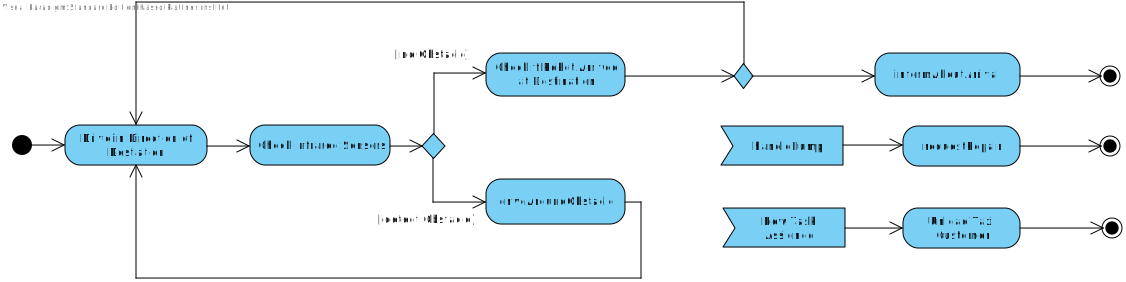
\includegraphics[width=1\textwidth]{img/7-1-methode_driveToDestination}
			\caption{Aktivitätsdiagramm zur Methode \texttt{driveToDestination}}
			\label{AktivitaetDriveToDestination}
			\end{figure}

			Wenn diese Methode aufgerufen wird, macht die \textit{RobotUnit} sich auf den Weg zur 
			übergebenen \textit{Destination}. Wenn die \textit{RobotUnit} an dieser \textit{Destination} 
			angekommen ist, wird die \texttt{arrive}-Methode des übergebenen \textit{ArrivalHandlers} ausgeführt. Wenn es sich bei der \textit{Destination} nicht um einen \textit{Charger} handelte, wird darin insbesondere über die von uns definierte Schnittstelle \textit{IArrivalNotifivation} der \textit{Server} über die Ankunft benachrichtigt. 
			Wenn sich ein \textit{Obstacle} auf dem Weg befindet, wird die Methode \texttt{driveAroundObstacle} 
			aufgerufen, bis das \textit{Obstacle} umfahren wurde.
			
			Abbildung \ref{AktivitaetDriveToDestination} zeigt ein entsprechendes Aktivitätsdiagramm.

			%7.1.2.2    -driveAroundObstacle(destination: Destination): void
			\paragraph{Beschreibung der Methode \texttt{driveAroundObstacle}}
			\begin{figure}[H]
			\centering
			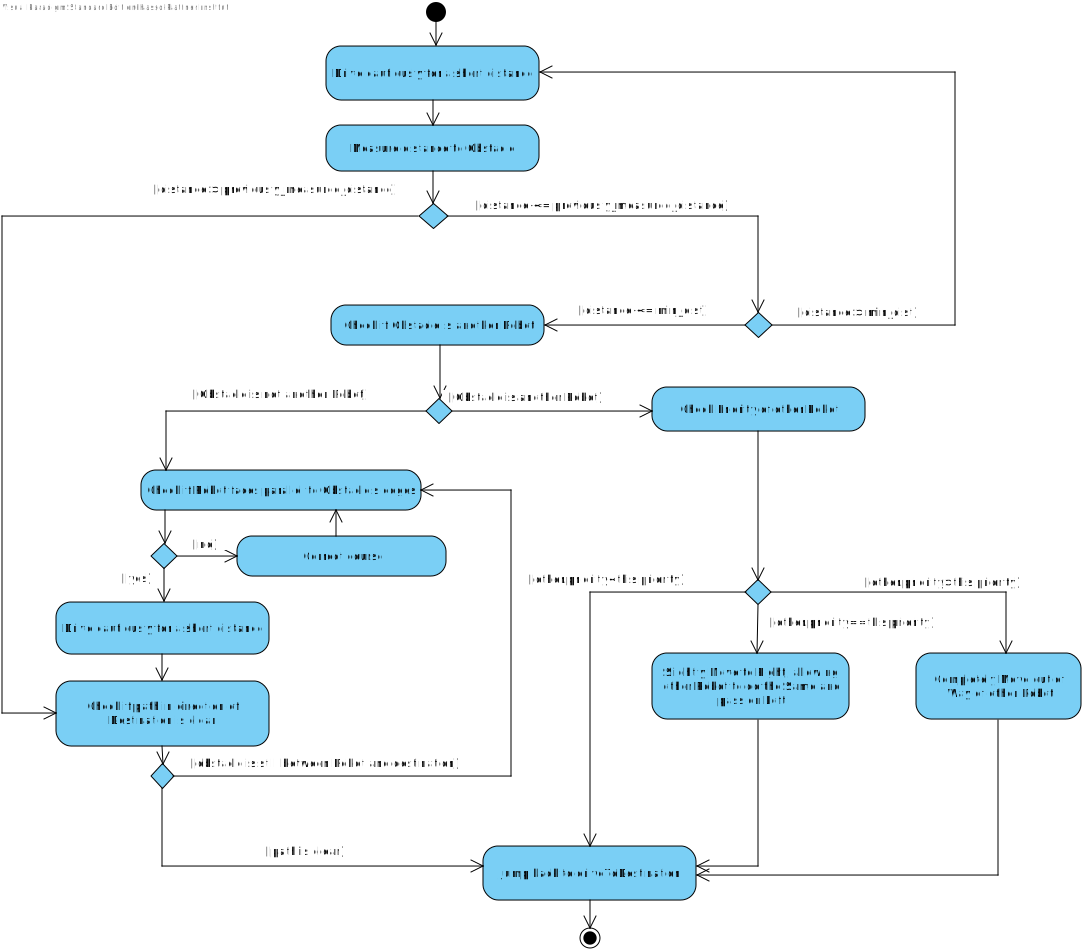
\includegraphics[width=0.95\textwidth]{img/1-Entwurf-7-driveAroundObstacle}
			\caption{Aktivitätsdiagramm zur Beschreibung der Methode \texttt{driveAroundObstacle}}
			\label{AktivitätDriveAroundObstacle}
			\end{figure}

			Diese Methode wird von \texttt{driveToDestination} mit der Position eines \textit{Obstacles} aufgerufen, 
			wenn ein \textit{Obstacle} zu umfahren ist. 
			Im Spezialfall, dass es sich bei dem \textit{Obstacle} um eine andere \textit{RobotUnit} handelt, merken dies beide. Wenn die beiden \textit{RobotUnits} gerade \textit{Tasks} mit der gleichen Priorität ausführen, weichen beide leicht nach rechts aus, und fahren anschließend aneinander vorbei. So nehmen beide einen ungefähr gleichen Umweg in kauf. Wenn eine \textit{RobotUnit} höher priorisiert ist als die andere, so weicht die \textit{RobotUnit} mit der niedrigeren Priorität komplett aus. So werden Krankenhaustransporte nie durch andere \textit{RobotUnits} verzögert.
			Im Allgemeinen entscheidet sich die \emph{RobotUnit} zunächst, ob er links oder rechts an dem \textit{Obstacle} vorbeifährt, 
			und hält sich dann mithilfe seiner Sensoren immer auf einem bestimmten Abstand zum Hindernis, bis zwischen 
			\textit{Obstacle} und der Luftlinie zur \textit{Destination} genug Platz für die \textit{RobotUnit} ist.
			
			Abbildung \ref{SequenzDriveAroundObstacle} zeigt ein entsprechendes Sequenzdiagramm. 
			Dabei ist \texttt{min\_dist} eine vorher festgelegte Konstante, welche die Mindestdistanz, die die \textit{RobotUnit} halten muss, wenn sie an einem \textit{Obstacle} vorbeifährt, speichert.
	
\pagebreak
	
%7.2 Paket Server
\subsection{Paket \textit{Server}}
%\begin{figure}[H]
%	\centering
%	\includegraphics[width=0.6\textwidth]{../images/Paketdetails.png}
%	\caption{\textcolor{blue}{HIER KOMMT DAS Server - PAKETDIAGRMAM HIN}}
%	\label{Paketdetails}
%	\end{figure}
	Im Folgenden werden die wichtigen Klassen des Pakets \textit{Server} 
	und ihre zugehörigen Methoden sowie ihre Interaktion untereinander beschrieben. 


	%7.2.1 TaskSystem
	\subsubsection{Beschreibung der Klasse \textit{TaskQueue}}
	
	Diese Klasse ist für die Verwaltung von \textit{Tasks} auf dem \textit{Server} zuständig. Prinzipiell ist hier eine Queue implementiert, welche aber noch über zusätzliche Funktionen, wie z.B \texttt{addTop} und \texttt{remove} verfügt. Ziel dieser Datenstruktur ist es, die Wartezeiten für mögliche Taxikunden fair zu handhaben und die Verteilung an die \textit{RobotUnits} vorzunehmen.
	
			\paragraph{Beschreibung der Methode \texttt{add}}		
			\begin{figure}[H]
			\centering
			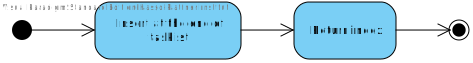
\includegraphics[width=0.95\textwidth]{img/add}
			\caption{Aktivitätsdiagramm zur Beschreibung der Methode \texttt{add}}
			\label{SequenzQueueAdd}
			\end{figure}
			
			Die Methode \texttt{add} dient dazu neue Tasks in die Warteliste einzufügen.
			
			\paragraph{Beschreibung der Methode \texttt{addTop}}		
%			\begin{figure}[H]
%			\centering
%			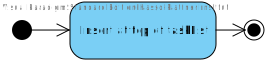
\includegraphics[width=0.95\textwidth]{img/addTop}
%			\caption{Sequenzdiagramm zur Beschreibung der Methode \texttt{addTop}}
%			\label{SequenzQueueAddTop}
%			\end{figure}			
			
			Mit der Methode \texttt{addTop} können \textit{Tasks} in die Queue hinzugefügt werden, die davor schon aktiv von einer \textit{RobotUnit} bearbeitet wurden, dann aber durch einen Defekt dessen neu verteilt werden müssen. 
			Die Besonderheit dieser \textit{Tasks} ist, dass sie an den Anfang der Queue hinzugefügt werden müssen.
				
			\paragraph{Beschreibung der Methode \texttt{poll}}		
			\begin{figure}[H]
			\centering
			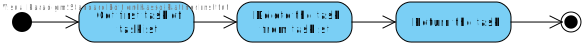
\includegraphics[width=0.95\textwidth]{img/2-Entwurf-poll}
			\caption{Aktivitätsdiagramm zur Beschreibung der Methode \texttt{poll}}
			\label{SequenzQueuePoll}
			\end{figure}			
			
			Die Methode \texttt{poll} gibt den nächsten zu bearbeitenden Task zurück und entfernt diesen aus der Queue.
				
			\paragraph{Beschreibung der Methode \texttt{remove}}		
			\begin{figure}[H]
			\centering
			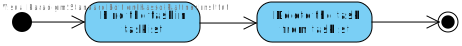
\includegraphics[width=0.95\textwidth]{img/2-Entwurf-remove}
			\caption{Aktivitätsdiagramm zur Beschreibung der Methode \texttt{remove}}
			\label{SequenzQueueRemove}
			\end{figure}			
			
			Die Methode \texttt{remove} entfernt einen spezifischen Task aus der Queue.
			
	%7.2.2 RobotControlSystem
	\subsubsection{Beschreibung der Klasse \textit{VirtualRobotManager}}
			\paragraph{Beschreibung der Methode \texttt{handleArrival}}
			\begin{figure}[H]
			\centering
			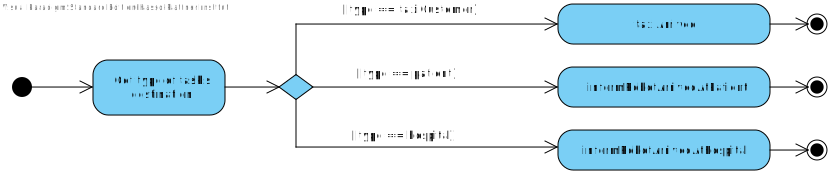
\includegraphics[width=0.95\textwidth]{img/HandleArrival}
			\caption{Aktivitätsdiagramm zur Beschreibung der Methode \texttt{handleArrival}}
			\label{SequenzQueuePoll}
			\end{figure}	
			Diese Methode wird immer dann aufgerufen, wenn der \textit{Server} eine \textit{Message} von einer \textit{RobotUnit} erhält, welche von ihm über das von uns definierte Interface \textit{IArrivalNotification} gesandt wurde. Da der \textit{Server} eingespeichert hat, welchen \textit{Task} die \textit{RobotUnit} gerade ausführt, müssen keine Parameter übergeben werden, sondern der \textit{Server} kann einfach nachschauen, welcher Typ von \textit{Destination} gerade erreicht wurde. Je nach Typ wird dann eine Benachrichtigung an die zugehörigen \textit{Customers} gesendet. Bei einem Taxiauftrag wird keine Nachricht an den Taxikunden geschickt, wenn dieser sein Ziel erreicht. Laut Aufgabenstellung ist eine Taxifahrt mit Erreichen der \textit{Destination} des Taxikunden sofort beendet, ohne dass weitere Benachrichtigungen an den Taxikunden geschickt werden müssen.
			
			
			%7.2.1.1	~chooseRobot(destination: Destination): void
			\paragraph{Beschreibung der Methode \texttt{chooseRobotUnit}}
						\begin{figure}[H]
			\centering
			\includegraphics[width=0.95\textwidth]{img/2-Analyse-7-Choose_Robot}
			\caption{Aktivitätsdiagramm zur Beschreibung der Methode \texttt{chooseRobotUnit}}
			\label{ChooseRobotActivity}
			\end{figure}			
			
			Die Methode \texttt{chooseRobotUnit} wählt für den aktuell eingegangenen \emph{Task} eine \emph{RobotUnit} aus. 
			Dazu fragt es die Sensorwerte derjenigen \textit{RobotUnits} ab, die gerade nicht mit einem Krankenhausauftrag beschäftigt sind. Diese haben nämlich höchste Priorität und können sowieso keinen anderen \textit{Task} erhalten. Danach wird die private Methode \texttt{selectBestMatch} mit der Liste der erhaltenen Sensordaten ausgeführt, welche den am besten passendsten \textit{Robot} für den aktuellen \textit{Task} berechnet.
				

			
			\paragraph{Beschreibung der Methode \texttt{selectBestMatch}}
			\begin{figure}[H]
			\centering
			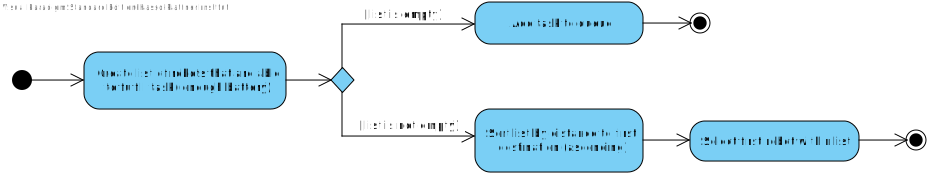
\includegraphics[width=0.95\textwidth]{img/2-Entwurf-SelectBestMatch}
			\caption{Aktivitätsdiagramm zur Beschreibung der Aktivität \texttt{selectBestMatch}}
			\label{SelectBestMatchActivity}
			\end{figure}
			Diese private Methode ist eine Untermethode von \texttt{chooseRobotUnit}. Dabei werden die erhaltenen Sensordaten der \textit{RobotUnits} nach dem zu vergebenen \textit{Task} ausgewertet. Die wichtigste Bedingung ist, dass der Akku der zugehörigen \textit{RobotUnits} ausreicht, um die gesamte Distanz zu schaffen. Das nächste Auswahlkriterium ist, dass die \textit{RobotUnitss} aktuell unbeschäftigt sind. Schließlich wird danach ausgewählt, wie lange die \textit{RobotUnitss} brauchen würden, um die erste \textit{Destination} dieses \textit{Tasks} zu erreichen.

			\paragraph{Beschreibung der Methode \texttt{notifyRepairService}}
			Wenn eine \textit{RobotUnit} nach einem Zusammenstoß defekt ist, teilt sie dies dem \textit{Server} unter Verwendung seiner Methode \texttt{requestRepair} mit.	Daraufhin erstellt der \textit{Server} einen neuen  \textit{Task}, der am Unfallort der \textit{RobotUnits} beginnt. Der \textit{Customer}, der an Bord der verunglückten \textit{RobotUnits} war, wird also nicht im Stich gelassen. Der neue \textit{Task} wird mit der Methode \texttt{addTopOfType} in die \textit{TaskQueue} eingefügt, um die Wartezeit dieses \textit{Customers} zu minimieren. Daraufhin benachrichtigt der \textit{Server} einen System-externen Servicedienst, und übergibt diesem die Position des Unfallorts. Nach unserer Annahme aus der Analyse wird die dort verunglückte \textit{RobotUnit} dann nach einer endlichen Zeit wieder vom System benutzbar sein.
			
			
			
	\subsubsection{Beschreibung der Klasse \textit{VirtualRobotUnit}}
	Die Klasse \textit{VirtualRobotUnit} ist die Umsetzung der Remote-Procedure-Calls von der Seite des \textit{Servers}. Diese Klasse implementiert die Methoden der von uns in 3. beschriebenen Interfaces \textit{ITask} und \textit{ISensorData}. Da diese Klasse auch die Repräsentation der \textit{RobotUnit} auf dem \textit{Server} ist, werden hier auch Zustand der zugehörigen \textit{RobotUnit}, insbesondere aktuell auszuführenden \textit{Task}, gespeichert. Alle Methoden dieser Klasse werden im \textit{Server} aufgerufen und Verfassen zunächst eine \textit{Message}, welche dann über die \textit{IWlanAdapter}-Schnittstelle verschickt werden und daraufhin die zugehörigen Lokalen Methoden auf den \textit{RobotUnits} aufgerufen werden.
	
			\paragraph{Beschreibung der Methode \texttt{assignTask}}
			Mit dieser Methode teilt der \textit{Server} einem \textit{VirtualRobot} einen neuen \textit{Task} zu, der dann von der zugehörigen \textit{RobotUnit} ausgeführt wird. Auf dem zugehörigen \textit{Robot} wird dafür die Methode \texttt{setTask} aufgerufen.
			
			\paragraph{Beschreibung der Methode \texttt{continueTask}}
			Diese Methode wird zum Beispiel dann aufgerufen, wenn der \textit{Server} die Nachricht erhalten hat, dass sich der \textit{Customer} nun an Bord der \textit{RobotUnits} befindet. Daraufhin wird eine \textit{Message} an den zu dieser \textit{VirtualRobotUnit} zugehörigen \textit{RobotUnit} geschickt, der sie wissen lässt, dass er die nächste \textit{Destination} in seinem aktuellen \textit{Task}			
			
			\paragraph{Beschreibung der Methode \texttt{getSensorData}}
			Der \textit{Server} möchte im Rahmen von \texttt{chooseRobotUnit} Informationen über den Akkustand und die Position von allen \textit{RobotUnits} erhalten. Dazu wird auf jeder \textit{VirtualRobotUnit} diese Methode aufgerufen, bei der über die \textit{IWlanAdapter}-Schnittstelle eine entsprechende \textit{Message} an den jeweils zugehörigen \textit{Robot} geschickt wird. Diese \textit{RobotUnits} rufen dann die Methode \texttt{readSensors} auf.
